\documentclass[../distribution_theory_notes.tex]{subfiles}
\begin{document}
\section{Aula 23 - 15 de Novembro, 2024}
\subsection{Motivações}
\begin{itemize}
	\item Soluções fundamentais dos operadores clássicos;
	\item Operador de Laplace;
	\item Operador de Cauchy--Riemann.
\end{itemize}

\subsection{Soluções Fundamentais dos Operadores Clássicos}
Se
\[
	P(D)=\sum\limits_{|\alpha|\leq m}a_{\alpha}\partial^{\alpha}
\]
é um operador diferencial parcial linear com coeficientes constantes, uma \textbf{solução fundamental} de \(P(D)\) é uma distribuição \(E\in\mathcal{D}'(\mathbb{R}^{n})\) tal que
\[
	P(D)E=\delta.
\]
Sabemos que, nessas condições, se \(E\in L_{\mathrm{loc}}^{1}(\mathbb{R}^{n})\), então, para toda \(\varphi\in\mathcal{C}_{c}^{\infty}(\mathbb{R}^{n})\), vale a representação
\[
	\varphi(x)=\int_{\mathbb{R}^{n}}E(x-y)P(D)\varphi(y)\,dy,
	\qquad x\in\mathbb{R}^{n}.
\]

Queremos hoje apresentar e confirmar as soluções fundamentais canônicas dos operadores de Laplace e de Cauchy--Riemann. O que não faremos nesta aula será a ``dedução'' do que nos leva a considerar os candidatos que apresentaremos (isso poderia ser feito posteriormente com o auxílio da Transformada de Fourier). Nosso ponto de partida será o Teorema de Stokes, a partir do qual deduziremos a Segunda Identidade de Green, necessária para o caso do operador de Laplace, e a Fórmula de Integração por Partes, que usaremos no caso de Cauchy--Riemann.

\subsection{Operador de Laplace}
O \textbf{operador de Laplace} em \(\mathbb{R}^{n}\) é
\[
	\Delta=\sum\limits_{j=1}^{n}\frac{\partial^{2}}{\partial x_{j}^{2}}.
\]
Nós nos concentraremos no caso \(n\geq 3\), deixando o caso \(n=2\) para ser tratado nos exercícios.

\begin{lemma*}[Segunda Identidade de Green]
	Seja \(\Omega\subset\mathbb{R}^{n}\) um aberto com fronteira regular. Para todas \(u,v\in\mathcal{C}^{2}(\overline{\Omega})\), vale a igualdade
	\[
		\int_{\Omega}(u\Delta v-v\Delta u)\,dx
		=
		\int_{\partial\Omega}
		\left(
		u\frac{\partial v}{\partial\nu}
		-v\frac{\partial u}{\partial\nu}
		\right)d\sigma,
	\]
	em que
	\[
		\frac{\partial f}{\partial\nu}\coloneqq\nabla f\cdot\nu,
	\]
	sendo \(\nu\) o vetor normal unitário que aponta para fora de \(\Omega\), normal a \(\partial\Omega\), e \(d\sigma\) o elemento de volume da fronteira \(\partial\Omega\), isto é, a integral de superfície. \(\square\)
\end{lemma*}

\begin{tcolorbox}[
		skin=enhanced,
		title=Observação,
		fonttitle=\bfseries,
		colframe=black,
		colbacktitle=cyan!75!white,
		colback=cyan!15,
		colbacklower=black,
		coltitle=black,
		drop fuzzy shadow,
	]
	Dizer que \(\Omega\) é um aberto com fronteira regular significa que \(\overline{\Omega}\) é uma superfície compacta com bordo de dimensão \(n\), tal que
	\[
		\Omega=\operatorname{int}(\overline{\Omega}),
	\]
	e de classe \(\mathcal{C}^{1}\). Nesse caso, o bordo da superfície \(\overline{\Omega}\) coincide com a fronteira topológica de \(\Omega\).
\end{tcolorbox}

Consideremos
\[
	E_{0}:\mathbb{R}^{n}\setminus\{0\}\longrightarrow\mathbb{R},
	\qquad
	E_{0}(x)=|x|^{2-n},
	\qquad n\geq 3,
\]
e calculemos suas derivadas parciais. Temos:
\begin{align*}
	\text{(I)}\qquad
	\frac{\partial |x|}{\partial x_{j}}
	 & =\frac{x_{j}}{|x|},\; j=1,2,\ldots,n;                                              \\[0.4em]
	\text{(II)}\qquad
	\frac{\partial E_{0}}{\partial x_{j}}(x)
	 & =\frac{\partial}{\partial x_{j}}\bigl(|x|^{2-n}\bigr)
	=(2-n)|x|^{1-n}\frac{\partial |x|}{\partial x_{j}}
	=(2-n)x_{j}|x|^{-n};                                                                  \\[0.4em]
	\text{(III)}\qquad
	\frac{\partial^{2}E_{0}}{\partial x_{j}^{2}}(x)
	 & =(2-n)\frac{\partial}{\partial x_{j}}\bigl(x_{j}|x|^{-n}\bigr)                     \\
	 & =(2-n)\left[|x|^{-n}+x_{j}(-n)|x|^{-n-1}\frac{\partial |x|}{\partial x_{j}}\right] \\
	 & =(2-n)\left[|x|^{-n}-n x_{j}^{2}|x|^{-n-2}\right].
\end{align*}
Consequentemente,
\begin{align*}
	\Delta E_{0}
	 & =(2-n)\left[
		\sum\limits_{j=1}^{n}|x|^{-n}
		-n|x|^{-n-2}\sum\limits_{j=1}^{n}x_{j}^{2}
	\right]                                               \\
	 & =(2-n)\left[n|x|^{-n}-n|x|^{-n-2}|x|^{2}\right]=0.
\end{align*}
Ou seja, \(E_{0}\) é harmônica em \(\mathbb{R}^{n}\setminus\{0\}\).

\begin{tcolorbox}[
		skin=enhanced,
		title=Observação,
		fonttitle=\bfseries,
		colframe=black,
		colbacktitle=cyan!75!white,
		colback=cyan!15,
		colbacklower=black,
		coltitle=black,
		drop fuzzy shadow,
	]
	Se
	\[
		S_{r}^{n-1}\coloneqq\{x\in\mathbb{R}^{n}:|x|=r\},
	\]
	então \(\sigma(S_{r}^{n-1})\), a área de \(S_{r}^{n-1}\), satisfaz
	\[
		\sigma(S_{r}^{n-1})=r^{n-1}\sigma(S^{n-1}).
	\]
	Em particular,
	\[
		\sigma(S_{r}^{1})=r\sigma(S^{1})=2\pi r
	\]
	quando \(n=2\).
\end{tcolorbox}

Agora, notemos que \(E_{0}\in L_{\mathrm{loc}}^{1}(\mathbb{R}^{n})\), de acordo com a mudança de variáveis em coordenadas polares. Usaremos o seguinte fato.

\begin{lemma*}
	Se \(f(x)=g(|x|)\), \(x\in\mathbb{R}^{n}\), com \(f\) mensurável positiva ou \(f\in L^{1}(\mathbb{R}^{n})\), então
	\[
		\int_{\mathbb{R}^{n}}f(x)\,dx
		=\sigma(S^{n-1})\int_{0}^{\infty}g(r)r^{n-1}\,dr.
	\]
\end{lemma*}

Com isso, vemos que
\begin{align*}
	\int_{B(0,1)}|x|^{2-n}\,dx
	 & =\sigma(S^{n-1})\int_{0}^{1}r^{2-n}r^{n-1}\,dr \\
	 & =\sigma(S^{n-1})\int_{0}^{1}r\,dr<\infty.
\end{align*}
Naturalmente, por ser contínua em \(\mathbb{R}^{n}\setminus\{0\}\), \(E_{0}\in L^{1}(K)\) para todo compacto \(K\Subset\mathbb{R}^{n}\setminus\{0\}\), e isso confirma que
\[
	E_{0}\in L_{\mathrm{loc}}^{1}(\mathbb{R}^{n}).
\]

Nessas condições, \(E_{0}\in\mathcal{D}'(\mathbb{R}^{n})\), e podemos calcular seu Laplaciano. Com efeito, dada \(\varphi\in\mathcal{C}_{c}^{\infty}(\mathbb{R}^{n})\), temos, pelo Teorema da Convergência Dominada de Lebesgue,
\begin{align*}
	\langle\Delta E_{0},\varphi\rangle
	 & =\langle E_{0},\Delta\varphi\rangle
	=\int_{\mathbb{R}^{n}}E_{0}(x)\Delta\varphi(x)\,dx \\
	 & =\lim_{\varepsilon\to0^{+}}
	\int_{F_{\varepsilon}}E_{0}(x)\Delta\varphi(x)\,dx,
\end{align*}
em que
\[
	F_{\varepsilon}
	\coloneqq
	\{x\in\mathbb{R}^{n}:\varepsilon\leq|x|\leq R\},
\]
onde \(R>0\) foi escolhido de modo que
\[
	\operatorname{supp}(\varphi)\subset B(0,R).
\]
\begin{figure}[H]
	\begin{center}
		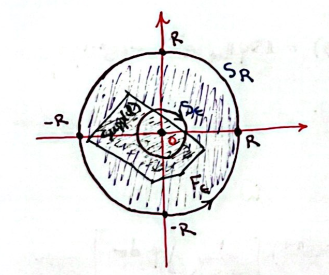
\includegraphics[height=0.4\textheight, width=0.4\textwidth, keepaspectratio]{./Images/23_supp_out.png}
	\end{center}
	\caption{Uma porção do suporte de \(\varphi \) fica fora da \(F_{\varepsilon }\).}
\end{figure}

Usando a Segunda Identidade de Green com \(\varphi\) no lugar de \(u\) e \(E_{0}\) no lugar de \(v\), e observando que \(F_{\varepsilon}\) é um domínio regular, podemos escrever
\[
	\int_{F_{\varepsilon}}(\varphi\Delta E_{0}-E_{0}\Delta\varphi)\,dx
	=
	\int_{\partial F_{\varepsilon}}
	\left(
	\varphi\frac{\partial E_{0}}{\partial\nu}
	-E_{0}\frac{\partial\varphi}{\partial\nu}
	\right)d\sigma.
\]
Como \(E_{0}\) é harmônica em \(\mathbb{R}^{n}\setminus\{0\}\), temos \(\Delta E_{0}=0\) em \(F_{\varepsilon}\), e a igualdade acima se escreve
\begin{align*}
	-	\int_{F_{\varepsilon}}E_{0}\Delta\varphi\,dx
	 & =\int_{\partial F_{\varepsilon}}
	\left(
	\varphi\frac{\partial E_{0}}{\partial\nu}
	-E_{0}\frac{\partial\varphi}{\partial\nu}
	\right)d\sigma                      \\
	 & =\int_{S_{R}}
	\left(
	\varphi\frac{\partial E_{0}}{\partial\nu}
	-E_{0}\frac{\partial\varphi}{\partial\nu}
	\right)d\sigma
	-
	\int_{S_{\varepsilon}}
	\left(
	\varphi\frac{\partial E_{0}}{\partial\nu}
	-E_{0}\frac{\partial\varphi}{\partial\nu}
	\right)d\sigma.
\end{align*}
Aqui, \(\partial F_{\varepsilon}=S_{\varepsilon}\cup S_{R}\); em \(S_{R}\), o vetor normal aponta radialmente para fora, enquanto em \(S_{\varepsilon}\) a orientação é a oposta. Como \(\operatorname{supp}(\varphi)\subset B(0,R)\), a integral sobre \(S_{R}\) é nula, e sendo \(E_{0}(x)=| x |^{2}\), para \(\sigma\in S_{\varepsilon}\), temos
\[
	E_{0}(\sigma)=\varepsilon^{2-n}
\]
e
\begin{align*}
	\frac{\partial E_{0}}{\partial\nu}(x)
	 & =\nabla E_{0}(x)\cdot\frac{x}{|x|}
	=\sum\limits_{j=1}^{n}\frac{\partial E_{0}}{\partial x_{j}}(x)\frac{x_{j}}{|x|} \\
	 & =(2-n)|x|^{-n-1}\sum\limits_{j=1}^{n}x_{j}^{2}
	=(2-n)|x|^{1-n},
\end{align*}
de modo que
\[
	\frac{\partial E_{0}}{\partial\nu}(\sigma)
	=(2-n)\varepsilon^{1-n},
	\qquad \sigma\in S_{\varepsilon}.
\]
Logo,
\begin{align*}
	-	\int_{F_{\varepsilon}}E_{0}(x)\Delta\varphi(x)\,dx
	 & =-\int_{S_{\varepsilon}}
	\left(
	\varphi(2-n)\varepsilon^{1-n}
	-\varepsilon^{2-n}\frac{\partial\varphi}{\partial\nu}
	\right)d\sigma                                                              \\
	 & =-(2-n)\frac{1}{\varepsilon^{n-1}}\int_{S_{\varepsilon}}\varphi\,d\sigma
	+\varepsilon^{2-n}\int_{S_{\varepsilon}}\frac{\partial\varphi}{\partial\nu}\,d\sigma.
\end{align*}

Para a segunda parcela,
\begin{align*}
	\varepsilon^{2-n}
	\int_{S_{\varepsilon}}
	\left|\frac{\partial\varphi}{\partial\nu}\right|d\sigma
	 & \leq
	\varepsilon^{2-n}\|\nabla\varphi\|_{\infty}\int_{S_{\varepsilon}}d\sigma \\
	 & =\|\nabla\varphi\|_{\infty}\,
	\varepsilon^{2-n}\varepsilon^{n-1}\sigma(S^{n-1})                        \\
	 & =\varepsilon\,\|\nabla\varphi\|_{\infty}\sigma(S^{n-1})
	\stackrel{\varepsilon\to0^{+}}{\longrightarrow}0.
\end{align*}

A primeira parcela envolve
\begin{align*}
	\frac{1}{\varepsilon^{n-1}}\int_{S_{\varepsilon}}\varphi\,d\sigma
	 & =\sigma(S^{n-1})
	\left[
		\frac{1}{\varepsilon^{n-1}\sigma(S^{n-1})}
		\int_{S_{\varepsilon}}\varphi\,d\sigma
	\right]             \\
	 & =\sigma(S^{n-1})
	\left[
		\frac{1}{\sigma(S_{\varepsilon})}
		\int_{S_{\varepsilon}}\varphi\,d\sigma
		\right]
	\stackrel{\varepsilon\to0^{+}}{\longrightarrow}
	\sigma(S^{n-1})\varphi(0).
\end{align*}
Ou seja,
\[
	\lim_{\varepsilon\to0^{+}}
	\int_{F_{\varepsilon}}E_{0}\Delta\varphi\,dx
	=(2-n)\sigma(S^{n-1})\varphi(0).
\]
Concluímos que
\[
	\langle\Delta E_{0},\varphi\rangle
	=(2-n)\sigma(S^{n-1})\varphi(0),
\]
e, portanto,
\[
	E(x)\coloneqq
	\frac{1}{(2-n)\sigma(S^{n-1})}|x|^{2-n}
\]
é uma solução fundamental \(L_{\mathrm{loc}}^{1}\) do Laplaciano.

\begin{tcolorbox}[
		skin=enhanced,
		title=Observação,
		fonttitle=\bfseries,
		colframe=black,
		colbacktitle=cyan!75!white,
		colback=cyan!15,
		colbacklower=black,
		coltitle=black,
		drop fuzzy shadow,
	]
	Se \(n=3\), então \(\sigma(S^{2})=4\pi\) e
	\[
		E(x)=-\frac{1}{4\pi|x|}
	\]
	é o potencial gravitacional no vácuo.
\end{tcolorbox}

\subsection{Operador de Cauchy--Riemann}
Em \(\mathbb{R}^{2}\cong\mathbb{C}\), consideramos o operador de Cauchy--Riemann
\[
	\frac{\partial}{\partial\overline{z}}
	=\frac{1}{2}\left(
	\frac{\partial}{\partial x}
	+i\frac{\partial}{\partial y}
	\right).
\]
Como antes, enunciamos uma consequência do Teorema de Stokes que permite a forma geral da integração por partes.

\begin{lemma*}[Integração por Partes]
	Seja \(\Omega\subseteq\mathbb{R}^{n}\) um domínio compacto com fronteira regular. Se \(f,g\in\mathcal{C}^{1}(\overline{\Omega})\) e \(\nu:\partial\Omega\to\mathbb{R}^{n}\) é o campo de vetores normais que aponta para fora de \(\Omega\), com
	\[
		\nu(\sigma)=\bigl(\nu_{1}(\sigma),\ldots,\nu_{n}(\sigma)\bigr),
		\qquad \sigma\in\partial\Omega,
	\]
	então
	\[
		\int_{\Omega}f\frac{\partial g}{\partial x_{j}}\,dx
		=
		\int_{\partial\Omega}(fg)\nu_{j}\,d\sigma
		-
		\int_{\Omega}\frac{\partial f}{\partial x_{j}}g\,dx,
		\qquad j=1,2,\ldots,n.
	\]
\end{lemma*}

\begin{tcolorbox}[
		skin=enhanced,
		title=Observação,
		fonttitle=\bfseries,
		colframe=black,
		colbacktitle=cyan!75!white,
		colback=cyan!15,
		colbacklower=black,
		coltitle=black,
		drop fuzzy shadow,
	]
	Se \(f\) ou \(g\) pertence a \(\mathcal{C}_{c}^{1}(\Omega)\), então
	\[
		\int_{\partial\Omega}fg\,\nu_{j}\,d\sigma=0,
	\]
	e recuperamos a fórmula usada para definir a derivada em \(\mathcal{D}'\).
\end{tcolorbox}

Consideremos
\[
	E_{0}(z)\coloneqq\frac{1}{z},
	\qquad z=x+iy\neq0,
	\qquad x,y\in\mathbb{R}.
\]
Essa é apenas uma forma ``compacta'' de escrever a função
\[
	E_{0}(x,y)
	=\frac{x}{x^{2}+y^{2}}-i\frac{y}{x^{2}+y^{2}},
\]
pois
\[
	\frac{1}{z}=\frac{\overline{z}}{|z|^{2}}.
\]
Calculemos as derivadas parciais de \(E_{0}\). Observando primeiro que
\[
	f(x,y)=\log(x^{2}+y^{2}),
\]
temos
\begin{align*}
	\text{(I)}\qquad \frac{\partial f}{\partial x}  =\frac{2x}{x^{2}+y^{2}} & =2\operatorname{Re}(E_{0}) \;\&\;\frac{\partial f}{\partial y} =\frac{2y}{x^{2}+y^{2}}=-2\operatorname{Im}(E_{0});                    \\[0.5em]
	\text{(II)}\qquad
	\frac{\partial}{\partial x}\left(\frac{x}{x^{2}+y^{2}}\right)
	                                                                        & =\frac{x^{2}+y^{2}-2x^{2}}{(x^{2}+y^{2})^{2}}
	=\frac{y^{2}-x^{2}}{(x^{2}+y^{2})^{2}};                                                                                                                                                                         \\[0.5em]
	\text{(III)}\qquad
	\frac{\partial}{\partial y}\left(\frac{y}{x^{2}+y^{2}}\right)
	                                                                        & =\frac{x^{2}-y^{2}}{(x^{2}+y^{2})^{2}};                                                                                               \\[0.5em]
	\text{(IV)}\qquad
	\frac{\partial}{\partial y}\left(\frac{x}{x^{2}+y^{2}}\right)
	                                                                        & =-\frac{2xy}{(x^{2}+y^{2})^{2}} \;\&\; \frac{\partial}{\partial x}\left(\frac{y}{x^{2}+y^{2}}\right) =-\frac{2xy}{(x^{2}+y^{2})^{2}}.
\end{align*}
As relações (I)--(III) mostram que \(f(x,y)=\log(x^{2}+y^{2})\) é harmônica em \(\mathbb{R}^{2}\setminus\{(0,0)\}\). Já sabíamos que \(f\) é a parte real da função holomorfa \(2\log z\), \(z\in\mathbb{C}\).

A fórmula de mudança de variáveis também mostra que \(E_{0}\in L_{\mathrm{loc}}^{1}(\mathbb{R}^{2})\), porque
\begin{align*}
	\iint_{B(0,1)}|E_{0}(x,y)|\,dx\,dy
	 & =\sigma(S^{1})\int_{0}^{1}\frac{1}{r}r\,dr \\
	 & =\sigma(S^{1})<\infty,
\end{align*}
e \(E_{0}\) é contínua em \(\mathbb{R}^{2}\setminus\{0\}\). Assim,
\(E_{0}\in\mathcal{D}'(\mathbb{R}^{2}),\) e podemos calcular \(\partial E_{0}/\partial\overline{z}\) em \(\mathcal{D}'(\mathbb{R}^{2})\).

Dada
\[
	\Phi(x,y)=\varphi(x,y)+i\psi(x,y),
	\qquad
	\varphi,\psi\in\mathcal{C}_{c}^{\infty}(\mathbb{R}^{2};\mathbb{R}),
\]
temos
\begin{align*}
	\left\langle\frac{\partial E_{0}}{\partial\overline{z}},\Phi\right\rangle
	 & =-\left\langle E_{0},\frac{\partial\Phi}{\partial\overline{z}}\right\rangle \\
	 & =-\iint_{\mathbb{R}^{2}}E_{0}(x,y)
	\frac{\partial\Phi}{\partial\overline{z}}(x,y)\,dx\,dy                         \\
	 & =-\lim_{\varepsilon\to0^{+}}
	\iint_{F_{\varepsilon}}E_{0}(x,y)
	\frac{\partial\Phi}{\partial\overline{z}}(x,y)\,dx\,dy,
\end{align*}
pelo Teorema da Convergência Dominada de Lebesgue, onde, como anteriormente,
\[
	F_{\varepsilon}=\{(x,y):\varepsilon\leq |z|\leq R\}
\]
para \(R\) suficientemente grande.

Calculemos o integrando explicitamente. Primeiramente,
\begin{align*}
	\frac{\partial\Phi}{\partial\overline{z}}
	 & =\frac{\partial\varphi}{\partial\overline{z}}
	+i\frac{\partial\psi}{\partial\overline{z}}             \\
	 & =\frac{1}{2}\left(\frac{\partial\varphi}{\partial x}
	+i\frac{\partial\varphi}{\partial y}\right)
	+\frac{i}{2}\left(\frac{\partial\psi}{\partial x}
	+i\frac{\partial\psi}{\partial y}\right)                \\
	 & =\frac{1}{2}\left(\frac{\partial\varphi}{\partial x}
	-\frac{\partial\psi}{\partial y}\right)
	+\frac{i}{2}\left(\frac{\partial\varphi}{\partial y}
	+\frac{\partial\psi}{\partial x}\right).
\end{align*}
Portanto,
\begin{align*}
	E_{0}\frac{\partial\Phi}{\partial\overline{z}}
	 & =\frac{1}{2}
	\left[\frac{x}{x^{2}+y^{2}}-i\frac{y}{x^{2}+y^{2}}\right]
	\left[
		\left(\frac{\partial\varphi}{\partial x}-\frac{\partial\psi}{\partial y}\right)
		+i\left(\frac{\partial\varphi}{\partial y}+\frac{\partial\psi}{\partial x}\right)
	\right]               \\
	 & =\frac{1}{2}\left[
		\frac{x}{x^{2}+y^{2}}
		\left(\frac{\partial\varphi}{\partial x}-\frac{\partial\psi}{\partial y}\right)
		+\frac{y}{x^{2}+y^{2}}
		\left(\frac{\partial\varphi}{\partial y}+\frac{\partial\psi}{\partial x}\right)
	\right]               \\
	 & \quad+
	\frac{i}{2}\left[
		\frac{x}{x^{2}+y^{2}}
		\left(\frac{\partial\varphi}{\partial y}+\frac{\partial\psi}{\partial x}\right)
		-\frac{y}{x^{2}+y^{2}}
		\left(\frac{\partial\varphi}{\partial x}-\frac{\partial\psi}{\partial y}\right)
		\right].
\end{align*}

Comecemos integrando por partes a parte real, sem o fator \(1/2\):
\begin{align*}
	 & \iint_{F_{\varepsilon}}
	\left(
	\frac{x}{x^{2}+y^{2}}\frac{\partial\varphi}{\partial x}
	-\frac{x}{x^{2}+y^{2}}\frac{\partial\psi}{\partial y}
	+\frac{y}{x^{2}+y^{2}}\frac{\partial\varphi}{\partial y}
	+\frac{y}{x^{2}+y^{2}}\frac{\partial\psi}{\partial x}
	\right)dx\,dy                       \\
	 & =\int_{\partial F_{\varepsilon}}
	\left(
	\frac{x\varphi}{x^{2}+y^{2}}\nu_{x}
	-\frac{x\psi}{x^{2}+y^{2}}\nu_{y}
	+\frac{y\varphi}{x^{2}+y^{2}}\nu_{y}
	+\frac{y\psi}{x^{2}+y^{2}}\nu_{x}
	\right)d\sigma                      \\
	 & \quad-
	\iint_{F_{\varepsilon}}
	\left[
		\varphi\left(\frac{y^{2}-x^{2}}{|z|^{4}}\right)
		-\psi\left(\frac{-2xy}{|z|^{4}}\right)
		+\varphi\left(\frac{x^{2}-y^{2}}{|z|^{4}}\right)
		+\psi\left(\frac{-2xy}{|z|^{4}}\right)
		\right]dx\,dy.
\end{align*}
A integral dupla na última linha é nula, pelas relações (II)--(IV). A integral sobre a componente externa da fronteira também é nula, pois \(\varphi\) e \(\psi\) se anulam em \(S_{R}\). No círculo interno \(S_{\varepsilon}\), o normal exterior a \(F_{\varepsilon}\) aponta para dentro, isto é,
\[
	\nu=-\frac{(x,y)}{|z|}.
\]
Daí, a integral de fronteira reduz-se a
\begin{align*}
	-	\int_{S_{\varepsilon}}
	\left(
	\varphi\frac{x}{|z|^{2}}\frac{x}{|z|}
	-\psi\frac{xy}{|z|^{2}|z|}
	+\varphi\frac{y^{2}}{|z|^{2}|z|}
	+\psi\frac{xy}{|z|^{2}|z|}
	\right)d\sigma
	 & =-\int_{S_{\varepsilon}}
	\varphi\frac{x^{2}+y^{2}}{|z|^{3}}\,d\sigma                        \\
	 & =-\int_{S_{\varepsilon}}\frac{\varphi}{|z|}\,d\sigma            \\
	 & =-\int_{S_{\varepsilon}}\frac{\varphi}{\varepsilon}\,d\sigma    \\
	 & =-2\pi\left(
	\frac{1}{2\pi\varepsilon}\int_{S_{\varepsilon}}\varphi\,d\sigma
	\right)                                                            \\
	 & =-2\pi\left(
	\frac{1}{\sigma(S_{\varepsilon})}\int_{S_{\varepsilon}}\varphi\,d\sigma
	\right)                                                            \\
	 & \stackrel{\varepsilon\to0^{+}}{\longrightarrow}-2\pi\varphi(0).
\end{align*}
Desse modo,
\[
	\iint_{F_{\varepsilon}}
	\operatorname{Re}\left(
	E_{0}\frac{\partial\Phi}{\partial\overline{z}}
	\right)dx\,dy
	\stackrel{\varepsilon\to0^{+}}{\longrightarrow}
	-\pi\varphi(0).
\]
Analogamente, como exercício,
\[
	\iint_{F_{\varepsilon}}
	\operatorname{Im}\left(
	E_{0}\frac{\partial\Phi}{\partial\overline{z}}
	\right)dx\,dy
	\stackrel{\varepsilon\to0^{+}}{\longrightarrow}
	-\pi\psi(0).
\]
Juntando tudo, concluímos que
\begin{align*}
	\left\langle\frac{\partial E_{0}}{\partial\overline{z}},\Phi\right\rangle
	 & =-\lim_{\varepsilon\to0^{+}}
	\iint_{F_{\varepsilon}}E_{0}\frac{\partial\Phi}{\partial\overline{z}}\,dx\,dy \\
	 & =\pi\bigl(\varphi(0)+i\psi(0)\bigr)
	=\pi\Phi(0).
\end{align*}
Portanto,
\[
	E(z)\coloneqq\frac{1}{\pi}E_{0}(z)=\frac{1}{\pi z}
\]
é uma solução fundamental \(L_{\mathrm{loc}}^{1}(\mathbb{R}^{2})\) do operador \(\partial/\partial\overline{z}\).

\subsection{Apêndices}
\textbf{(1º)} O \textbf{Teorema da Divergência de Gauss--Ostrogradski} diz que, se \(\Omega\) é um domínio com \(\partial\Omega\) regular e
\[
	w=(w_{1},\ldots,w_{n})\in\mathcal{C}^{1}(\overline{\Omega}),
\]
então
\[
	\int_{\Omega}\operatorname{div}(w)\,dx
	=\int_{\partial\Omega}w\cdot\nu\,d\sigma,
\]
onde \(\nu:\partial\Omega\to\mathbb{R}^{n}\) é o campo normal que aponta para fora de \(\Omega\), e \(d\sigma\) é o elemento de volume, ou área, de superfície.

Em particular, se \(u,v\in\mathcal{C}^{2}(\overline{\Omega})\), pondo
\[
	w=u\nabla v,
\]
calculamos
\begin{align*}
	\operatorname{div}(w)
	 & =\sum\limits_{j=1}^{n}\frac{\partial}{\partial x_{j}}
	\left(u\frac{\partial v}{\partial x_{j}}\right)                 \\
	 & =\sum\limits_{j=1}^{n}\frac{\partial u}{\partial x_{j}}
	\frac{\partial v}{\partial x_{j}}
	+u\sum\limits_{j=1}^{n}\frac{\partial^{2}v}{\partial x_{j}^{2}} \\
	 & =\nabla u\cdot\nabla v+u\Delta v.
\end{align*}
Logo,
\[
	\int_{\Omega}(\nabla u\cdot\nabla v+u\Delta v)\,dx
	=\int_{\partial\Omega}w\cdot\nu\,d\sigma
	=\int_{\partial\Omega}u\frac{\partial v}{\partial\nu}\,d\sigma.
\]
Trocando os papéis de \(u\) e \(v\), encontramos
\[
	\int_{\Omega}(\nabla u\cdot\nabla v+v\Delta u)\,dx
	=\int_{\partial\Omega}v\frac{\partial u}{\partial\nu}\,d\sigma.
\]
Fazendo a primeira igualdade menos a segunda, obtemos
\[
	\int_{\Omega}(u\Delta v-v\Delta u)\,dx
	=\int_{\partial\Omega}
	\left(
	u\frac{\partial v}{\partial\nu}
	-v\frac{\partial u}{\partial\nu}
	\right)d\sigma.
\]

\textbf{(2º)} Se \(G\) é outra solução fundamental de \(\Delta\), então
\[
	\Delta(G-E)=0
\]
em \(\mathbb{R}^{n}\). Assim,
\[
	H=G-E
\]
é harmônica, logo
\[
	G=H+E,
\]
e essa é a expressão geral de uma solução fundamental de \(\Delta\), a menos da adição de uma função harmônica.

Analogamente, se \(G\) é uma solução fundamental de \(\partial/\partial\overline{z}\), então
\[
	G=U+\frac{1}{\pi z}
\]
para alguma função inteira
\[
	U:\mathbb{C}\longrightarrow\mathbb{C}.
\]
Isso só se confirma depois de mostrarmos que \(\Delta\) e \(\partial/\partial\overline{z}\) são \textit{hipoelípticos}.

\end{document}
